% Options for packages loaded elsewhere
\PassOptionsToPackage{unicode}{hyperref}
\PassOptionsToPackage{hyphens}{url}
%
\documentclass[a4paper,11pt,twoside,pdftex,draft]{article}
\usepackage{lmodern}
\usepackage{amssymb,amsmath}
\usepackage{ifxetex,ifluatex}
\ifnum 0\ifxetex 1\fi\ifluatex 1\fi=0 % if pdftex
  \usepackage[T1]{fontenc}
  \usepackage[utf8]{inputenc}
  \usepackage{textcomp} % provide euro and other symbols
\else % if luatex or xetex
  \usepackage{unicode-math}
  \defaultfontfeatures{Scale=MatchLowercase}
  \defaultfontfeatures[\rmfamily]{Ligatures=TeX,Scale=1}
\fi
% Use upquote if available, for straight quotes in verbatim environments
\IfFileExists{upquote.sty}{\usepackage{upquote}}{}
\IfFileExists{microtype.sty}{% use microtype if available
  \usepackage[]{microtype}
  \UseMicrotypeSet[protrusion]{basicmath} % disable protrusion for tt fonts
}{}
\makeatletter
\@ifundefined{KOMAClassName}{% if non-KOMA class
  \IfFileExists{parskip.sty}{%
    \usepackage{parskip}
  }{% else
    \setlength{\parindent}{0pt}
    \setlength{\parskip}{6pt plus 2pt minus 1pt}}
}{% if KOMA class
  \KOMAoptions{parskip=half}}
\makeatother
\usepackage{xcolor}
\IfFileExists{xurl.sty}{\usepackage{xurl}}{} % add URL line breaks if available
\IfFileExists{bookmark.sty}{\usepackage{bookmark}}{\usepackage{hyperref}}
\hypersetup{
  hidelinks,
  pdfcreator={LaTeX via pandoc}}
\urlstyle{same} % disable monospaced font for URLs
\usepackage{longtable,booktabs}
% Correct order of tables after \paragraph or \subparagraph
\usepackage{etoolbox}
\makeatletter
\patchcmd\longtable{\par}{\if@noskipsec\mbox{}\fi\par}{}{}
\makeatother
% Allow footnotes in longtable head/foot
\IfFileExists{footnotehyper.sty}{\usepackage{footnotehyper}}{\usepackage{footnote}}
\makesavenoteenv{longtable}
\usepackage{graphicx}
\makeatletter
\def\maxwidth{\ifdim\Gin@nat@width>\linewidth\linewidth\else\Gin@nat@width\fi}
\def\maxheight{\ifdim\Gin@nat@height>\textheight\textheight\else\Gin@nat@height\fi}
\makeatother
% Scale images if necessary, so that they will not overflow the page
% margins by default, and it is still possible to overwrite the defaults
% using explicit options in \includegraphics[width, height, ...]{}
\setkeys{Gin}{width=\maxwidth,height=\maxheight,keepaspectratio}
% Set default figure placement to htbp
\makeatletter
\def\fps@figure{htbp}
\makeatother
\setlength{\emergencystretch}{3em} % prevent overfull lines
\providecommand{\tightlist}{%
  \setlength{\itemsep}{0pt}\setlength{\parskip}{0pt}}
\setcounter{secnumdepth}{-\maxdimen} % remove section numbering


% Geometry for A4 layout like MS-Word defaults
\usepackage[left=2.54cm,top=2.54cm,bottom=2.54cm,right=2.54cm]{geometry}


\date{}

\begin{document}

CASAL2

Input File Specification

v2016.1

Author:

\emph{Scott Rasmussen}

\emph{Zaita}

\emph{scott.rasmussen@zaita.com}

Table of Contents

\protect\hyperlink{document-history}{Document History 3}

\protect\hyperlink{file-format-overview}{CASAL II Overview 3}

\protect\hyperlink{keywords-and-reserved-characters}{Supported Software
Requirements 3}

\protect\hyperlink{__RefHeading__140_571873561}{Development Environment
4}

\protect\hyperlink{operating-systems}{Operating Systems 4}

\protect\hyperlink{development-environment}{Development Environment 4}

\protect\hyperlink{windows}{Windows 4}

\protect\hyperlink{linux}{Linux 4}

\protect\hyperlink{both}{Both 4}

\protect\hyperlink{coding-style}{Coding Style 4}

\protect\hyperlink{high-level-design}{High-Level Design 5}

\protect\hyperlink{level-0-data-flow-diagram}{Level 0 Data-Flow-Diagram
5}

\protect\hyperlink{state-transition-diagram}{State-Transition Diagram 5}

\protect\hyperlink{software-components}{Software Components 6}

\protect\hyperlink{utilities-library}{Utilities Library 6}

\protect\hyperlink{configuration-file-parser}{Configuration File Parser
6}

\protect\hyperlink{equation-parser}{Equation Parser 6}

\protect\hyperlink{minimisers}{Minimisers 6}

\protect\hyperlink{state-model}{State-Model 6}

\protect\hyperlink{plugin-architecture}{Plugin Architecture 7}

\protect\hyperlink{dynamic-library}{Dynamic-Library 7}

\protect\hyperlink{command-line-executable}{Command-Line Executable 7}

\protect\hyperlink{equation-parser-1}{Equation Parser 7}

\protect\hyperlink{opencl-kernel}{OpenCL Kernel 8}

\hypertarget{document-history}{%
\section{Document History}\label{document-history}}

\begin{longtable}[]{@{}llll@{}}
\toprule
\endhead
Version & Description & Author & Date\tabularnewline
1.0 & \emph{Initial version - Draft} & S.Rasmussen &
20/11/2012\tabularnewline
V2016.1 & \emph{Updated for CASAL2 information and actual func} &
S.Rasmussen & 20/01/2116\tabularnewline
& & &\tabularnewline
& & &\tabularnewline
\bottomrule
\end{longtable}

\hypertarget{file-format-overview}{%
\section{\texorpdfstring{File Format Overview
}{File Format Overview }}\label{file-format-overview}}

The file format used for CASAL2 is based on the formats used for CASAL
and SPM. It's a standard text file that contains definitions organised
into blocks.

Without exception, every object specfified in a configuration file is
part of a block. At the top level blocks have a one-to-one relationships
with components in the system.

Example:

\begin{longtable}[]{@{}l@{}}
\toprule
\endhead
\begin{minipage}[t]{0.97\columnwidth}\raggedright
@block1 label

parameter value

parameter value\_1 value 2

@block2 label

parameter value

table table\_name

column\_1 column\_2

data\_1 data\_2

data\_3 data\_4

end\_table\strut
\end{minipage}\tabularnewline
\bottomrule
\end{longtable}

Some general notes about writing configuration files:

\begin{enumerate}
\def\labelenumi{\arabic{enumi}.}
\item
  1. Whitespace can be used freely. Tabs and spaces are both accepted
\item
  2. A block ends only at the beginning of a new block or end of final
  configuration file
\item
  You can include another configuration file from anywhere
\item
  Included files are placed inline, so you can continue a block in a new
  file
\item
  The configuration files support inline declarations of objects
\end{enumerate}

\hypertarget{keywords-and-reserved-characters}{%
\section{Keywords And Reserved
Characters}\label{keywords-and-reserved-characters}}

In order to allow efficient creation of input files CASAL2's file format
contains special keywords and characters that cannot be used for labels
etc.

\hypertarget{block-definitions}{%
\subsection{'@' Block Definitions}\label{block-definitions}}

Every new block in the configuration file must start with a block
definition character. The reserved character for this is the '@'
character.

Example:

\begin{longtable}[]{@{}l@{}}
\toprule
\endhead
\begin{minipage}[t]{0.97\columnwidth}\raggedright
@block1 \textless label\textgreater{}

type \textless type\textgreater{}

@block2 \textless label\textgreater{}

type \textless type\textgreater{}\strut
\end{minipage}\tabularnewline
\bottomrule
\end{longtable}

\hypertarget{type-keyword}{%
\subsection{'Type' Keyword}\label{type-keyword}}

The 'type' keyword is used for declaring the sub-type of a defined
block. Any block object that has multiple sub-types will use the type
keyword.

Example:

\begin{longtable}[]{@{}l@{}}
\toprule
\endhead
\begin{minipage}[t]{0.97\columnwidth}\raggedright
@block1 \textless label\textgreater{}

type \textless sub\_type\textgreater{}

@block2 \textless label\textgreater{}

type \textless sub\_type\textgreater{}\strut
\end{minipage}\tabularnewline
\bottomrule
\end{longtable}

\hypertarget{single-line-comment}{%
\subsection{\# (Single-Line Comment)}\label{single-line-comment}}

Comments are supported in the configuration file in either single-line
(to end-of-line) or multi-line

Example:

\begin{longtable}[]{@{}l@{}}
\toprule
\endhead
\begin{minipage}[t]{0.97\columnwidth}\raggedright
@block \textless label\textgreater{}

type \textless sub\_type\textgreater{} \#Descriptive comment

\#parameter \textless value\_1\textgreater{} -- This whole line is
commented out

parameter \textless value\_1\textgreater{}
\#\textless value\_2\textgreater(value\_2 is commented out)\strut
\end{minipage}\tabularnewline
\bottomrule
\end{longtable}

\hypertarget{multi-line-comment}{%
\subsection{\{ \} (Multi-Line Comment)}\label{multi-line-comment}}

Multiple line comments are supported by surrounding the comments in \{
and \}

Example:

\begin{longtable}[]{@{}l@{}}
\toprule
\endhead
\begin{minipage}[t]{0.97\columnwidth}\raggedright
@block \textless label\textgreater{}

type \textless sub\_type\textgreater{}

parameter \textless value\_1\textgreater{}

parameter \textless value\_1\textgreater{}
\textless value\_2\textgreater{}

\{ Do not load this process

@block \textless label\textgreater{}

type \textless sub\_type\textgreater{}

parameter \textless value\_1\textgreater{}

parameter \textless value\_1\textgreater{}
\textless value\_2\textgreater{}

\}\strut
\end{minipage}\tabularnewline
\bottomrule
\end{longtable}

\hypertarget{range-specifier}{%
\subsection{':' (Range Specifier)}\label{range-specifier}}

The range specifier allows you to specify a range of values at once
instead of having to input them manually. Ranges can be either
incremental or decremental.

Example:

\begin{longtable}[]{@{}l@{}}
\toprule
\endhead
\begin{minipage}[t]{0.97\columnwidth}\raggedright
@process my\_recruitment\_process

type constant\_recruitment

years\_to\_run 1999:2009 \#With range specifier

@process my\_mortality\_process

type natural\_mortality

years\_to\_run 2000 2001 2002 2003 2004 2005 2006 2007 \#Without range
specifier\strut
\end{minipage}\tabularnewline
\bottomrule
\end{longtable}

\hypertarget{list-specifier}{%
\subsection{',' (List Specifier)}\label{list-specifier}}

When a parameter supports multiple values in a single entry you can use
the list specifier to supply multiple values as a single parameter.

Example:

\begin{longtable}[]{@{}l@{}}
\toprule
\endhead
\begin{minipage}[t]{0.97\columnwidth}\raggedright
@categories

format sex.stage

names male,female.immature,mature \#With list specifier

@categories

format sex.stage

names male.immature male.mature female.immature female.mature \#Without
list specifier\strut
\end{minipage}\tabularnewline
\bottomrule
\end{longtable}

\hypertarget{table-and-end_table-keyword}{%
\subsection{'Table' and 'End\_Table'
Keyword}\label{table-and-end_table-keyword}}

The table keyword is used to define a table of information used as a
parameter. The line following the table declaration must contain a list
of columns to be used.

Following lines are rows of the table. Each row must have the same
number of values as the number of columns specified.

The table definition must end with the 'end\_table' keyword on it's own
line.

The first row of a table will be the name of the columns if required.

Example:

\begin{longtable}[]{@{}l@{}}
\toprule
\endhead
\begin{minipage}[t]{0.97\columnwidth}\raggedright
@block \textless label\textgreater{}

type \textless sub\_type\textgreater{}

parameter \textless value\_1\textgreater{}

table \textless table\_label\textgreater{}

\textless column\_1\textgreater{} \textless column\_2\textgreater{}
\textless column\_n\textgreater{}

\textless row1\_value1\textgreater{}
\textless row1\_value2\textgreater{}
\textless row1\_valueN\textgreater{}

\textless row2\_value1\textgreater{}
\textless row2\_value2\textgreater{}
\textless row2\_valueN\textgreater{}

end\_table\strut
\end{minipage}\tabularnewline
\bottomrule
\end{longtable}

\hypertarget{inline-declarations}{%
\subsection{{[} {]} (Inline Declarations)}\label{inline-declarations}}

When an object takes the label of a target object as a parameter this
can be replaced with an inline declaration. An inline declaration is a
complete declaration of an object one 1 line. This is designed to allow
the configuration writer to simplify the configuration writing process.

Example:

\begin{longtable}[]{@{}l@{}}
\toprule
\endhead
\begin{minipage}[t]{0.97\columnwidth}\raggedright
\#With inline declaration with label specified for time step

@model

time\_steps step\_one={[}type=iterative; processes=recruitment ageing{]}

\#With inline declaration with default label (model.1)

@model

time\_steps {[}type=iterative; processes=recruitment ageing{]}

\#Without inline declaration

@model

time\_steps step\_one

@time\_step step\_one

processes recruitment ageing\strut
\end{minipage}\tabularnewline
\bottomrule
\end{longtable}

\begin{enumerate}
\setcounter{enumi}{3}
\item ~
  \hypertarget{categories}{%
  \section{Categories}\label{categories}}

  The CASAL2 model is essentially a 2-dimensional model. The model
  partition is:

  Categories x Ages/Lengths.

  Each category supports the ability to have a different range of
  ages/lengths and accessibility during different time periods.

  Because each category is quite complicated the syntax for defining
  categories has been structured to allow complex definitions using a
  simple short-hand structure.

  The ``format'' parameter allows you to tell the model the structure of
  the category labels. By using a ``.'' (period) character between each
  segment we can utilise this later in the model to do short-hand
  lookups of categories.

  The ``names'' parameter is a list of the category names. The syntax of
  these names will need to match the ``format'' parameter so CASAL2 can
  organise and search on them. Using the ``list specifier'' and range
  characters we can shorten this parameter significantly.
\end{enumerate}

Example:

\begin{longtable}[]{@{}l@{}}
\toprule
\endhead
\begin{minipage}[t]{0.97\columnwidth}\raggedright
@categories

format sex.stage.tag

names male.immature.notag male.immature.2001 male.mature.notag
male.mature.2001

names male.immature \#Invalid: No tag information

names female \#Invalid: no stage of tag information

names female.immature.notag.1 \#Invalid: Extra format segment not
defined

names male,female.immature,mature.notag,2001:2005 \#OK!

\#Without short-hand. You'd have to write:

names male.immature.notag male.immature.2001 male.immature.2002
male.immature.2003 male.immature.2004 male.immature.2005
male.mature.notag male.mature.2001 male.mature.2002 male.mature.2003
male.mature.2004 male.mature.2005 female.immature.notag
female.immature.2001 female.immature.2002 female.immature.2003
female.immature.2004 female.immature.2005 female.mature.notag
female.mature.2001 female.mature.2002 female.mature.2003
female.mature.2004 female.mature.2005\strut
\end{minipage}\tabularnewline
\bottomrule
\end{longtable}

When we have specific data for a year in a category we don't want the
model to process this category during other years (or the initialisation
stages). We can define a list of years where each category will be
available, this will override the default of all years in the model. Any
category where you overwrite the default will no longer be accessible in
the initialisation phases.

\emph{Examples:}

\begin{longtable}[]{@{}l@{}}
\toprule
\endhead
\begin{minipage}[t]{0.97\columnwidth}\raggedright
@model

start\_year 1998

final\_year 2010

@categories

format sex.stage.tag

names male,female.immature,mature.notag,2001:2005 \#OK!

years tag=2001=1999:2003 tag=2005=2003:2007

\# Categories with the tag value ``2001'' will be available during years
1999, 2000, 2001, 2002 and 2003

\# Categories with the tag value ``2005'' will be available during the
years 2003, 2004, 2005, 2006, 2007\strut
\end{minipage}\tabularnewline
\bottomrule
\end{longtable}

\emph{Notes: Specifying a category more than once during this phase will
cause an error}

\begin{enumerate}
\item ~
  \hypertarget{operating-systems}{%
  \subsection{Operating Systems}\label{operating-systems}}

  Microsoft Windows 7 (x64)
\end{enumerate}

OpenSuSe 11.4 Celadon (x86\_64)

\begin{enumerate}
\setcounter{enumi}{1}
\item ~
  \hypertarget{development-environment}{%
  \subsection{Development Environment}\label{development-environment}}

  \emph{Note: It is expected that during the development of CASAL II
  some of these tools/libraries will be upgraded to more current
  versions as they are released.}

  \begin{enumerate}
  \item ~
    \hypertarget{windows}{%
    \subsubsection{Windows}\label{windows}}
  \end{enumerate}
\end{enumerate}

\begin{itemize}
\item
  TDM-GCC 4.6
  (\href{http://tdm-gcc.tdragon.net/}{{http://tdm-gcc.tdragon.net/}} )
\item
  Notepad++
  (\href{http://notepad-plus-plus.org/}{{http://notepad-plus-plus.org/}}
  )
\item
  AQTime3 -- Profiling
\item
  AMD Code Analyst
\item
  AMD App Profiler

  \begin{enumerate}
  \item ~
    \hypertarget{linux}{%
    \subsubsection{Linux}\label{linux}}
  \end{enumerate}
\end{itemize}

\begin{itemize}
\item
  GCC/G++ 4.5.1
\item
  Valgrind

  \begin{enumerate}
  \item ~
    \hypertarget{both}{%
    \subsubsection{Both}\label{both}}
  \end{enumerate}
\end{itemize}

\begin{itemize}
\item
  Eclipse Indigo
  (\href{http://www.eclipse.org/}{{http://www.eclipse.org/}} )
\item
  Boost 1.49.X (\href{http://www.boost.org/}{{http://www.boost.org/}} )
\item
  CMake 2.8.X (\href{http://www.cmake.org/}{{http://www.cmake.org/}} )
\item
  CLANG (\href{http://clang.llvm.org/}{{http://clang.llvm.org/}} )
\item
  GNU Debugger (GDB)

  \begin{enumerate}
  \item ~
    \hypertarget{coding-style}{%
    \subsection{Coding Style}\label{coding-style}}

    While it's going to be a step away from the style used for SPM,
    CASAL II will use the Google Coding style
    (\href{http://google-styleguide.googlecode.com/svn/trunk/cppguide.xml}{{http://google-styleguide.googlecode.com/svn/trunk/cppguide.xml}}
    ). Google provides a handy script to parse source code and highlight
    errors that do not match their coding style.

    Spelling of variable names, classes etc will all be done using
    British English.

    \emph{Note: The only deviation from this style is the use of *.cpp
    instead of *.cc for filename extensions.}
  \end{enumerate}
\end{itemize}

\begin{enumerate}
\setcounter{enumi}{4}
\item ~
  \hypertarget{high-level-design}{%
  \section{\texorpdfstring{\textbf{High-Level
  Design}}{High-Level Design}}\label{high-level-design}}

  \begin{enumerate}
  \item ~
    \hypertarget{level-0-data-flow-diagram}{%
    \subsection{Level 0
    Data-Flow-Diagram}\label{level-0-data-flow-diagram}}
  \end{enumerate}
\end{enumerate}

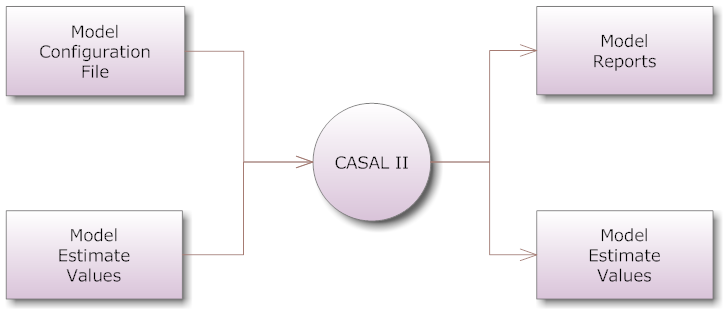
\includegraphics[width=6.0in,height=2.5in]{images/input_output.png}

\hypertarget{state-transition-diagram}{%
\subsection{State-Transition Diagram}\label{state-transition-diagram}}

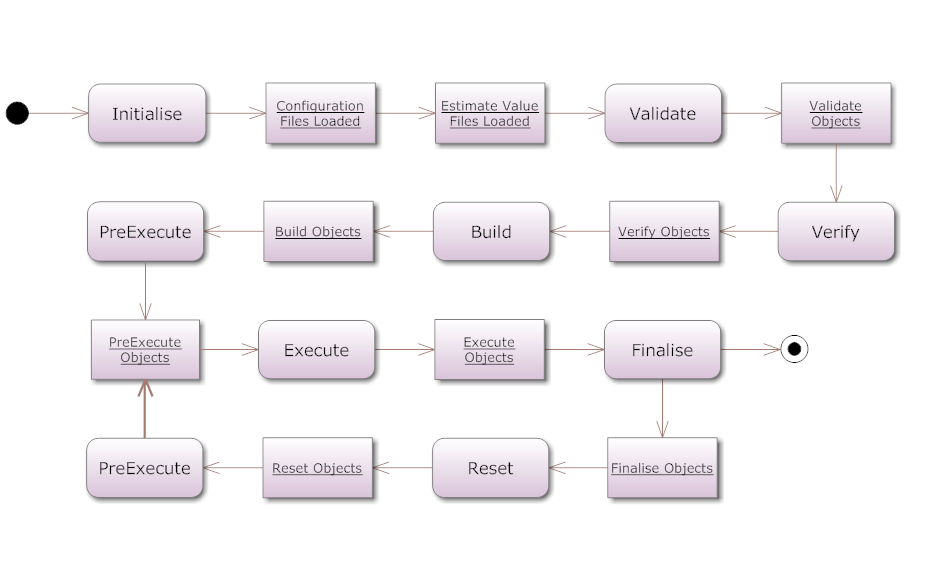
\includegraphics[width=6.0in,height=4.0in]{images/state_flow.png}

\begin{enumerate}
\setcounter{enumi}{5}
\item ~
  \hypertarget{state-descriptions}{%
  \section{State Descriptions}\label{state-descriptions}}

  \begin{enumerate}
  \item ~
    \hypertarget{initialise}{%
    \subsection{Initialise}\label{initialise}}
  \end{enumerate}
\end{enumerate}

The initialise state is the creation of components and parsing of
configuration files.

Tasks completed:

\begin{itemize}
\item
  Parse command line
\item
  Parse configuration file
\item
  Load plugins
\item
  Load estimate values from input files

  \begin{enumerate}
  \item ~
    \hypertarget{validate}{%
    \subsection{Validate}\label{validate}}
  \end{enumerate}
\end{itemize}

The validate state is used for checking user supplied options and
parameters to ensure they fit within hard-limits imposed by the
software.

\hypertarget{verify}{%
\subsection{Verify}\label{verify}}

The verification state is used to check the loaded configuration against
logical business rules. These are not hard-conditions imposed by the
system, but more logical conditions to ensure the user's configuration
file is going to produce a logical and useful result.

The amount of verification done can be customised through the
configuration file or command line options. This means verification is
not forced, and can optionally be ignored.

\hypertarget{build}{%
\subsection{Build}\label{build}}

The build phase is where the system will build relationships between
objects that rely on each other. Because validation has been completed,
each object in it's self-contained configuration is ok.

This phase generally assigns values to
shared\_ptrs\textless\textgreater{} for objects so they don't need to do
lookups of objects during execution phases.

\hypertarget{preexecute}{%
\subsection{PreExecute}\label{preexecute}}

The pre-execution phase is I don't know.

\hypertarget{execution}{%
\subsection{Execution}\label{execution}}

Das

\hypertarget{finalise}{%
\subsection{Finalise}\label{finalise}}

meh

\begin{enumerate}
\setcounter{enumi}{6}
\item ~
  \hypertarget{software-components}{%
  \section{Software Components}\label{software-components}}

  \begin{enumerate}
  \item ~
    \hypertarget{utilities-library}{%
    \subsection{Utilities Library}\label{utilities-library}}
  \end{enumerate}
\end{enumerate}

A stand-alone library for doing common functions within NIWA's modelling
applications will be developed for CASAL II.

This library will offer functionality like: Logging, Error handling,
double comparison, vector/map manipulation, string manipulation.

\hypertarget{configuration-file-parser}{%
\subsection{Configuration File Parser}\label{configuration-file-parser}}

A stand-alone library for loading and parsing configuration files for
NIWA's modelling applications will be developed for CASAL II. The code
from this will be mostly inherited from SPM and Random Station, but will
be largely re-factored to fit into a stand-alone library.

\hypertarget{equation-parser}{%
\subsection{Equation Parser}\label{equation-parser}}

CASAL II will use an open source equation parser with modifications to
make it compatible with ADMB. It's likely that two equation parsers will
exist within CASAL and a runtime decision will be made about which one
to picked based on the runtime parameters.

\hypertarget{minimisers}{%
\subsection{Minimisers}\label{minimisers}}

CASAL II will support 3 minimisers natively,

\begin{itemize}
\item
  DE Solver
\item
  GammaDiff
\item
  ADMB
\end{itemize}

While ADMB does need tight integration with CASAL II, the other 2
minimisers do not. These minimisers will be extracted into seperate
shared libraries and built as stand-alone components.

\hypertarget{state-model}{%
\subsection{State-Model}\label{state-model}}

As the state model for CASAL II is quite transferable across different
modelling applications it will be also extracted into it's own
stand-alone library.

\begin{enumerate}
\setcounter{enumi}{7}
\item ~
  \hypertarget{plugin-architecture}{%
  \section{Plugin Architecture}\label{plugin-architecture}}

  \begin{enumerate}
  \item ~
    \hypertarget{dynamic-library}{%
    \subsection{Dynamic-Library}\label{dynamic-library}}
  \end{enumerate}
\end{enumerate}

Developers with enough competence in C++ will be able to develop and
load their own plugins by building shared-libraries and specifying the
location of these within their configuration files.

An expected inclusion section of someone's plugin would be:

\#include \textless niwa/casal/process.h\textgreater{}

\#include \textless niwa/casal/selecvity.h\textgreater{}

class myNewProcess : public niwa::casal::process \{

public:

void validate() \{ \}

void build() \{ \}

void execute() \{ \}

\}

\emph{Difficulty for user to develop:} High

\emph{Execution speed:} Fast

\hypertarget{command-line-executable}{%
\subsection{Command-Line Executable}\label{command-line-executable}}

Some components of the application will be replacable with command line
applications that take specific arguments and return a single result
(e.g Selectivities/Layers).

A specification will be developed to allow people to build and specify
stand-alone executable based plugins for specific functionality within
CASAL II.

The upside to this approach is that the user can specify any type of
executable they wish, developed in any language, including
shell-scripts. The application will simply do an exec() call on that
object and intepret the result.

\emph{Difficulty for user to develop:} Low

\emph{Execution speed:} Slow

\hypertarget{equation-parser-1}{%
\subsection{Equation Parser}\label{equation-parser-1}}

CASAL II will have an inbuilt equation parser for handling equations
specified natively in the configuration file.

A valid example equation would be: 3\^{}x * 2

Where the user is able to bind 'x' to an internal parameter inside CASAL
II.

\emph{Difficulty for user to develop:} Low

\emph{Execution speed:} Slow

\hypertarget{opencl-kernel}{%
\subsection{OpenCL Kernel}\label{opencl-kernel}}

\emph{Note: This method was investigated, but at this point in time will
not persued. Keeping this information in here as a possible future
expansion of the software.}

An OpenCL kernel is a small file containing a vectorised C++ snippet of
code. When CASAL II starts it's able to load the kernel and compile it
against either a GPU (when one is present) or a CPU.

The speed benefits from using OpenCL on a GPU can be enormous because of
it's natively ability to work with multi-dimensional sets of data. Other
benefits are the ability to send someone a code-snippet and have CASAL
II compile it on the fly for execution, so platform indepdence is not an
issue.

The major downsides to this approach are development architecture and
difficulty. Developing an application around an OpenCL architecture
either has to be very modular or completely ingrained in the
application's structure. Difficulty in developing for OpenCL is very
high, especially among people who are not familiar with C++ syntax or
vector languages (e.g R/S+).

\emph{Difficulty for user to develop:} High

\emph{Execution speed:} Extremely Fast

\end{document}
